\lhead{\begin{tikzpicture}[remember picture, overlay]
    \node [anchor=100,inner sep=0] (imagenIZQUIERDA) at (current page header area.north){
\includegraphics[width=18cm]{img/Encabezado.PNG}};
    \end{tikzpicture}}
    \rhead{Avila-Hernández}
    \rfoot{\begin{tikzpicture}[remember picture, overlay]
    \node [anchor=140,inner sep=0] (imagenDERECHA) at (current page footer area.south){
\includegraphics[width=18cm]{img/Foot.PNG}};
    \end{tikzpicture}}
    %----------------------------------------------------------------------------------------
    \lfoot{ \thepage}
    % \renewcommand{\labelenumi}{\alph{enumi}.)} 
    %----------------------------------------------------------------------------------------
    %----------------------------------------------------------------------------------------
    %	TITLE SECTION
    %----------------------------------------------------------------------------------------
    
    \setlength{\droptitle}{-5\baselineskip} % Move the title up
    \title{\textbf{Estudio de tiempos y movimientos en el ensamble de un circuito electrónico utilizando diferentes métodos para su optimización}} % Article title
    
     \author{ 
     \textsc{Avila-Hernández, Diego}\\ 
    %  Afiliación:
     \texttt{ Instituto Tecnológico de Querétaro } \\ 
     \texttt{ Tecnológico Nacional de México } \\ 
     \texttt{Querétaro, México}\\ 
     \texttt{l22140920@queretaro.tecnm.mx} 
     \and 
     \textsc{Ángeles-Hurtado, Luis Alberto}\\ 
    %  Afiliación:
     \texttt{ Instituto Tecnológico de Querétaro } \\ 
     \texttt{ Tecnológico Nacional de México } \\ 
     \texttt{Querétaro, México}\\ 
     \texttt{alb3rt0.ah@gmail.com} 
    }
    
    
    %----------------------------------------------------------------------------------------
    
    % \begin{document}
    
    % Print the title
    \maketitle
    \thispagestyle{fancy}
    
    %----------------------------------------------------------------------------------------
    %	ARTICLE CONTENTS
    %----------------------------------------------------------------------------------------
    
    % \section*{Resumen}
    % \textit{Palabras clave:}
    % El resumen (ancho de página) deberá contener entre 100 y 200 palabras tipo Adobe Devangari 11 puntos.
    
    \begin{abstract}
    \noindent 
    El resumen (ancho de página) deberá contener entre 100 y 200 palabras tipo Adobe Devangari 11 puntos.
    
    \end{abstract}
    % 
    % 
    \textbf{\textit{Palabras clave}}:
    
    % \begin{itemize}
        Estudio, Tiempos, Movimientos, Métodos, Optimización, Circuito. 
    % \end{itemize}
    % 
    % {First keyword should be the corresponding to the research area according with the authors guide. Maximum of 6 keywords.}
    % \keywords{First keyword should be the corresponding to the research area according with the authors guide. Maximum of 6 keywords.}
    
    \section{Introducción}
    
    \begin{itemize}
    % \item Estudio: Esfuerzo que pone el entendimiento aplicándose a conocer algo.
    % \item Tiempos: Magnitud física que permite ordenar la secuencia de los sucesos.
    % \item Movimientos: Acción y efecto de mover.
    % \item Ensamble: Unir, juntar, ajustar, especialmente piezas.
    % \item Circuito: Terreno comprendido dentro de un perímetro cualquiera.
    % \item Electrónico: Perteneciente o relativo a la electrónica.
    % \item Métodos: Modo de decir o hacer con orden.
    % \item Optimización: Buscar la mejor manera de realizar una actividad.
    \item Esfuerzo aplicado para ordenar la secuencia de los movimientos al unir, juntar y ajustar los materiales en un circuito electrónico llevando a cabo un conjunto de reglas o principios para encontrar la mejor manera de realizar la actividad.\cite{RAE}
    \end{itemize}
    
    % \begin{itemize}
            % \item Se debe exponer de manera concreta y en lenguaje sencillo : el tema, o lo(s) objeto (s) de estudio. 
            % \item Se deben de mencionar las metodologías más usadas muy brevemente. 
            % \item Se debe de señalar el avance en los últimos años.
            % \item Al final se debe hacer alusión al o lo(s) objetivos del proyecto de investigación.
            % \item Debe de tener Referencias científicas, URL, tesis, etc.
        % \end{itemize}
        % 
        % 
    \section{Justificación}
    
    \begin{itemize}
    \item En el mundo de hoy, hay una mayor demanda de productos electrónicos avanzados y eficientes, lo que hace necesario mejorar la eficiencia y la productividad en la fabricación mediante la aplicación de análisis detallados de los tiempos y movimientos. Estos análisis tienen como objetivo encontrar y eliminar desperdicios en el proceso de ensamblaje, utilizando el tiempo, los recursos y la energía de manera óptima para lograr la máxima efectividad.
    A nivel local y nacional, existe una creciente preocupación por el impacto ambiental de la fabricación de circuitos electrónicos. Los gobiernos pueden promover prácticas más sostenibles, como los estudios de tiempos y movimientos, como parte de una estrategia de desarrollo sostenible. Esto podría implicar programas de subsidios para empresas que adopten prácticas más respetuosas con el medio ambiente.
        % \item Debe de tener Referencias científicas, URL, tesis, etc.
    \end{itemize}
     % 
     % 
    \section{Descripción del problema}
    \begin{itemize}
        \item Se debe describir la desviación o diferencia del ``es'' con respecto al ``debe ser''.
        \item Se debe hacer alusión a la incógnita científica*.
        \item Debe de tener Referencias científicas, URL, tesis, etc.
    \end{itemize}
    
    \textbf{*La incógnita científica es el elemento cuya solución incrementa el conocimiento
    científico.}
    % 
    % 
    \section{Fundamentación teórica}
    
    Es la parte medular y de mayor discusión, deberá ser la fundamentación de la hipótesis, por tanto se deberá señalar claramente la razón de la suposición y fundamentación de la misma. Únicamente referencias científicas.
    \begin{itemize}
        \item Se debe de retomar el tema que se planteo en la introducción, pero ahora profundizando para clarificar la incógnita científica y se pueda plantear la hipótesis.
        \item Se debe de retomar la descripción del problema, pero ahora a profundidad del (los) objeto(s) de estudio.
        \item Se debe de profundizar en las metodologías que se ha usado para el estudio del tema.
        \item Referencias solo de artículos y libros científicos.
    \end{itemize}
    % 
    % 
    \section{Hipótesis}
    
    \begin{itemize}
    \item Utilizando los Sistemas de Tiempo Predeterminado es posible reducir el tiempo para obtener el valor esperado y la desviación estándar.
    Es la suposición con fundamento científico relativa a la solución del problema, necesidad o de cómo se aprovecha la oportunidad con la incógnita científica y se fundamenta con: 1. Una suposición (en afirmativo o negativo) y ésta deberá vincularse con:
    2. La fundamentación científica que deberá ser precisa 3. Una entidad de comparación para probar la suposición y
    4. La variable con que se califica o cuantifica la comparación o se prueba la hipótesis.
    
    % \begin{itemize}
        \item Se debe de identificar claramente la suposición científica
        \item Se debe de identificar claramente el fundamento científico
        \item Se debe identificar claramente la variable de respuesta
        \item Se debe identifican claramente las realidades o modelos contrastantes
        \item Se debe de establecer las variables asociadas, explicativas o que tienen relación funcional con la variable de respuesta
    \end{itemize}
    % 
    % 
    \section{Objetivo}
    
    \begin{itemize}
    \item Diseñar, mejorar e integrar sistemas productivos de bienes y servicios  aplicando tecnologías para su optimización.
    % Precisar la acción necesaria para probar la hipótesis. Dicha acción se establece mediante el uso de verbos activos y en infinitivo.
    % \begin{itemize}
        % \item Se debe establecer que se pretende probar la hipótesis
    \end{itemize}
    
    \subsection{Objetivos específicos }
    
    \begin{itemize}
    \item Diseñar, implementar y mejorar sistemas de trabajo para elevar la productividad.
    \item Determinar mediante los registros históricos el tiempo productivo y compararlo con otros métodos.
    % \begin{itemize}
        % \item Se debe establecer como un conjunto de acciones comunes para lograr el objetivo general
        % \item Se debe establecer como etapas para lograr el objetivo general
    \end{itemize}
    
    % Son actividades orientadas al cumplimiento del objetivo general. Se establecen con verbos activos en infinitivo. Son parte de la acción encaminada a probar la hipótesis. Éstos deben ser precisos, y en lo posible evitar aspectos metodológicos.
    % 
    % 
    \section{Cuerpo (Metodología, modelo matemático, etc.)}
    
    \begin{itemize}
    \item Metodología. Planificación y diseño del circuito: Antes de comenzar el ensamblaje, es crucial tener un diseño detallado del circuito. Esto implica la creación de un esquemático. Se deben seleccionar los componentes adecuados y asegurarse de tener todas las herramientas y materiales necesarios.
    Preparación de los componentes: Verificar que todos los componentes necesarios estén disponibles y en buenas condiciones. Organizar los componentes de acuerdo con el esquemático del circuito para facilitar su acceso durante el ensamblaje.
    Preparación del área de trabajo: Asegurarse de tener un espacio limpio y bien iluminado para realizar el ensamblaje. Utilizar una superficie antideslizante y herramientas adecuadas, por ejemplo para este proyecto se usan herramientas como un tapete profesional organizador de trabajo, un multicontacto, un cable USB-C, un potenciómetro 3541H-1-102L 1k, un módulo adaptador LCD 1602, un protoboard, resistencias 330 1/4 W y cables dupont. Como máquinas se utiliza el LCD 16X2 y el ESP32-C6-WROOM-1. 
    Ensamblaje de componentes: Sigue las especificaciones de cada componente. 
    Pruebas y depuración: Una vez que todos los componentes estén colocados correctamente, realiza pruebas para asegurarte de que el circuito funcione según lo previsto. Si encuentras algún problema, depura el circuito identificando y corrigiendo posibles errores de conexión o defectos en los componentes. 
    Documentación y análisis: Documenta todo el proceso de ensamblaje, incluidos los problemas encontrados y las soluciones aplicadas. Esto ayudará en futuros proyectos y facilitará la replicación del circuito. Además, realiza un análisis del tiempo dedicado a cada etapa del proceso para identificar áreas de mejora y compararlo con otros métodos de ensamblaje.
    Para generar la estrategia metodológica; comprendo los objetivos ya que esta va acorde a cada objetivo. El objetivo específico es determinar mediante los registros históricos el tiempo productivo y compararlo con otros métodos. Así durante la operación como analista mido con cronómetro y cámara de video, llevo a cabo la recopilación de datos y hago un análisis, interpreto los resultados, identifico las conclusiones clave y comunico mis resultados de manera clara y efectiva. Todo esto para que se determine el tiempo productivo para después compararlo con otros métodos.
    % Cada estrategia metodológica se establece acorde a cada objetivo, y por tanto deberá ser desglosada precisada y ordenada claramente. En consecuencia cada objetivo que se presentó en forma de verbo en infinitivo deberá determinar una estrategia en forma de adverbio. Ej. Desarrollar…Desarrollo. Son las actividades ordenadas que tienen como finalidad la prueba de la hipótesis. 
    
    % \begin{itemize}
        % \item Se debe establecer que se habrá de hacer, como, conque, y donde para obtener la información que permita probar la hipótesis.  
        % \item Se debe desglosar de acuerdo a los objetivos específicos.
        % \item Se debe establecer una estrategia metodológica por cada objetivo específico. De manera simplista se podría decir que se cambia el verbo en infinitivo por su respectivo adverbio.
        % \item En cada objetivo se debe describir que método, que materiales y que equipo se usará para conseguirlo.
        \item Véase los materiales que se presentan a continuación:Figura\ref{fig:multicontactoFigura}.\ref{fig:cableUSB-CFigura}.\ref{fig:potenciómetroFigura}.\ref{fig:lcdFigura}.\ref{fig:móduloAdaptadorLcdFigura}.\ref{fig:esp32Figura}.\ref{fig:protoboardFigura}.\ref{fig:resistenciaFigura}.\ref{fig:cableMHFigura}.\ref{fig:cableMMFigura}.\ref{fig:tapeteProfesionalOrganizadorDeTrabajoFigura}
        \item Véase hoja de registro \ref{anexo:hojaDeRegistro }.
        \item Véase ensamble de circuito electrónico \ref{anexo:ensambleDeCircuitoElectrónico}
    \end{itemize}
    % 
    % 
    \subsection{Materiales}
    \begin{figure}[H]
        \centering
        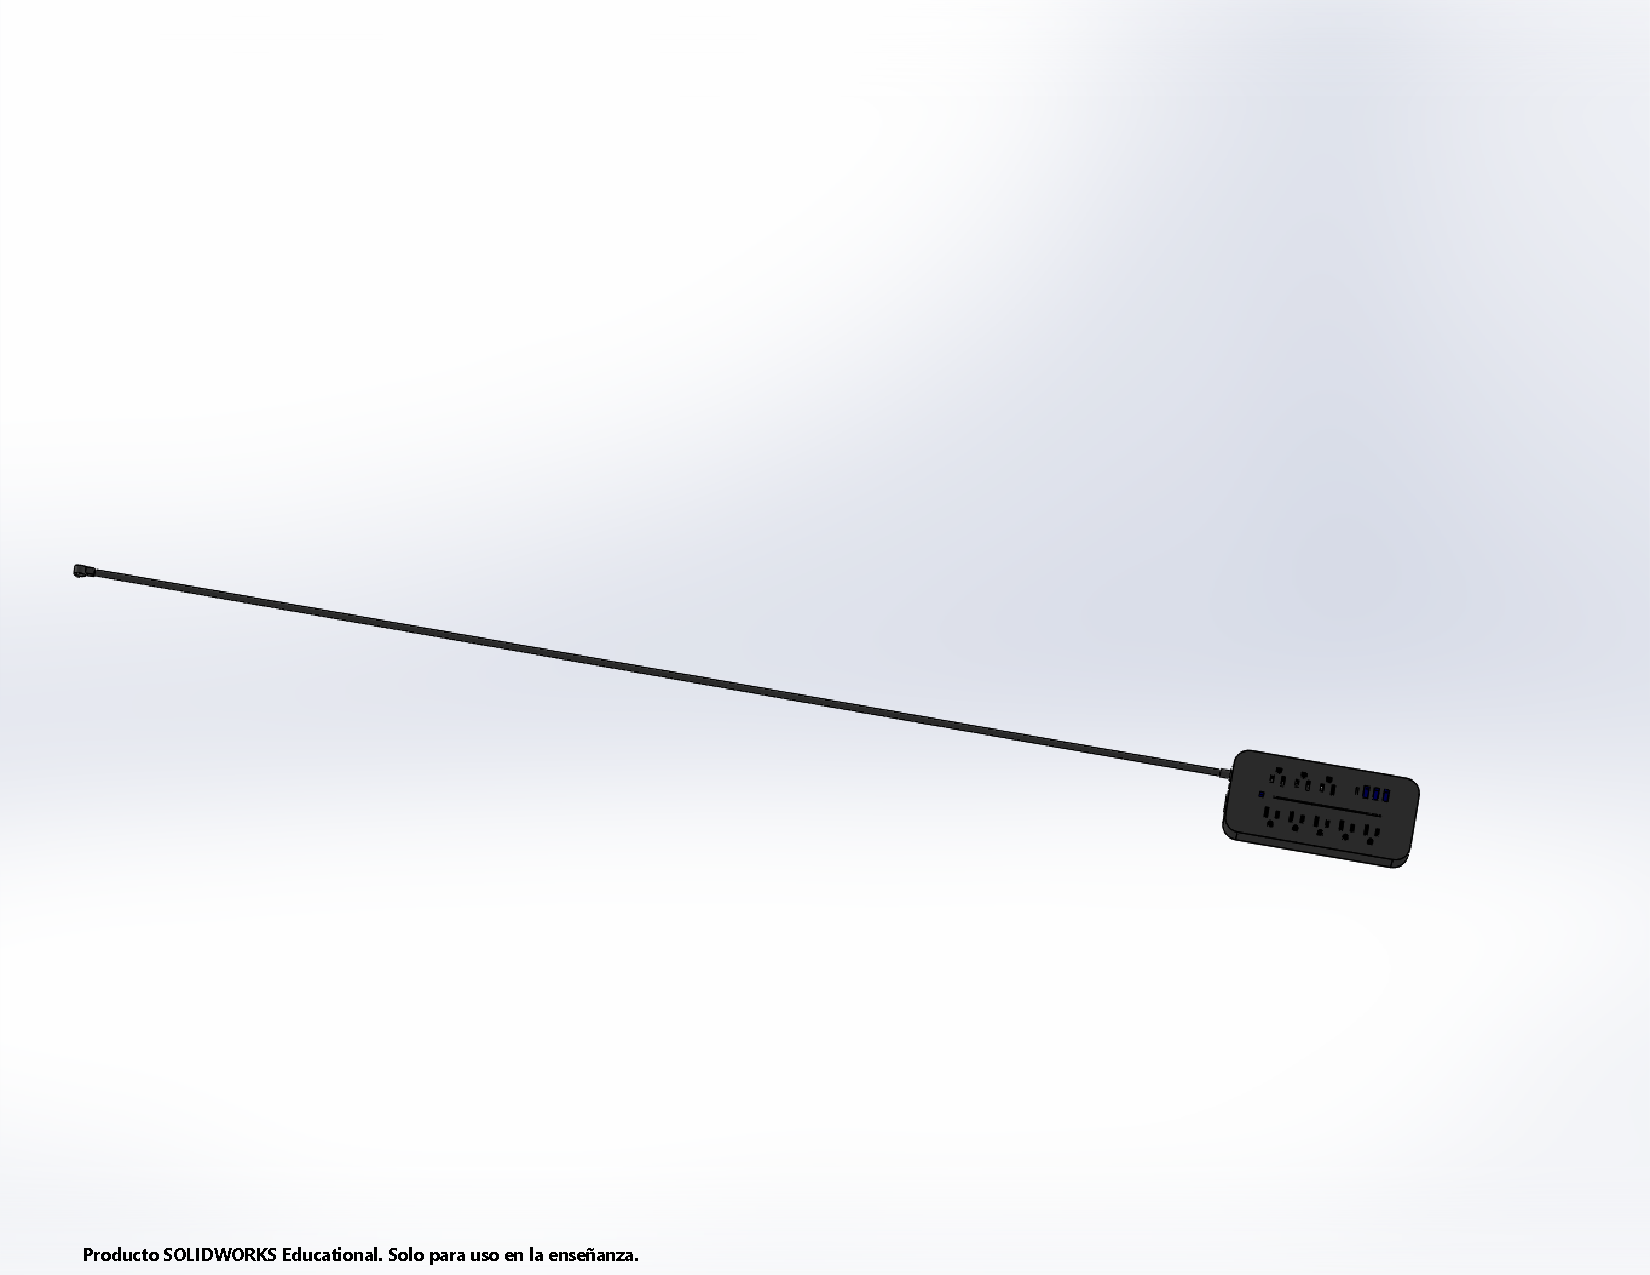
\includegraphics[trim = {5mm 50mm 15mm 60mm},clip,scale=0.2]{3/Img/multicontactoFigura.pdf}
        \caption{PC-01 Multicontacto}
        \label{fig:multicontactoFigura}
    \end{figure}
    % 
    % 
    \begin{figure}[H]
        \centering
        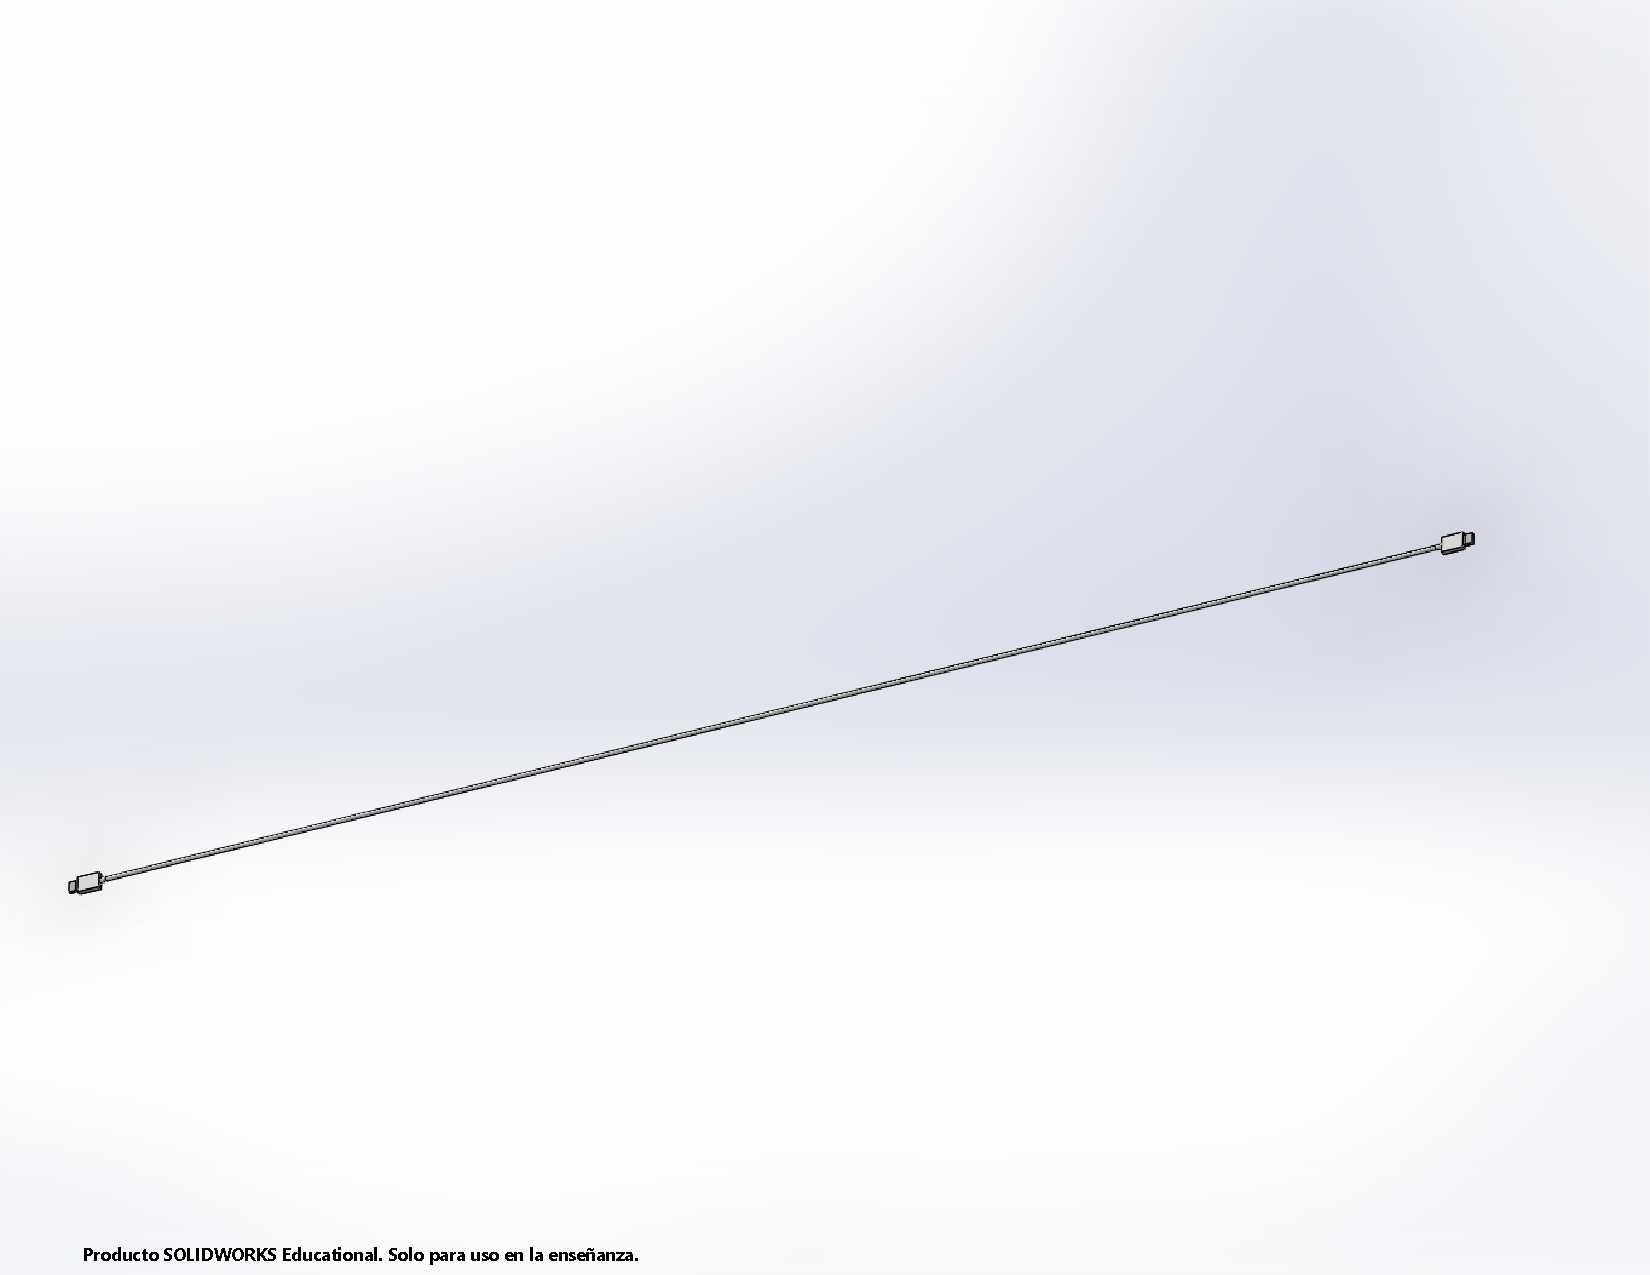
\includegraphics[trim = {1mm 50mm 1mm 60mm},clip,scale=0.2]{3/Img/cableUSB-CFigura.pdf}
        \caption{PC-02 Cable USB-C}
        \label{fig:cableUSB-CFigura}
    \end{figure}
    % 
    % 
    \begin{figure}[H]
        \centering
        \includegraphics[trim = {20mm 10mm 20mm 30mm},clip,scale=0.2]{3/Img/potenciómetroFigura.pdf}
        \caption{PC-03 Potenciómetro 3541H-1-102L 1k}
        \label{fig:potenciómetroFigura}
    \end{figure}
    % 
    % 
    \begin{figure}[H]
        \centering
        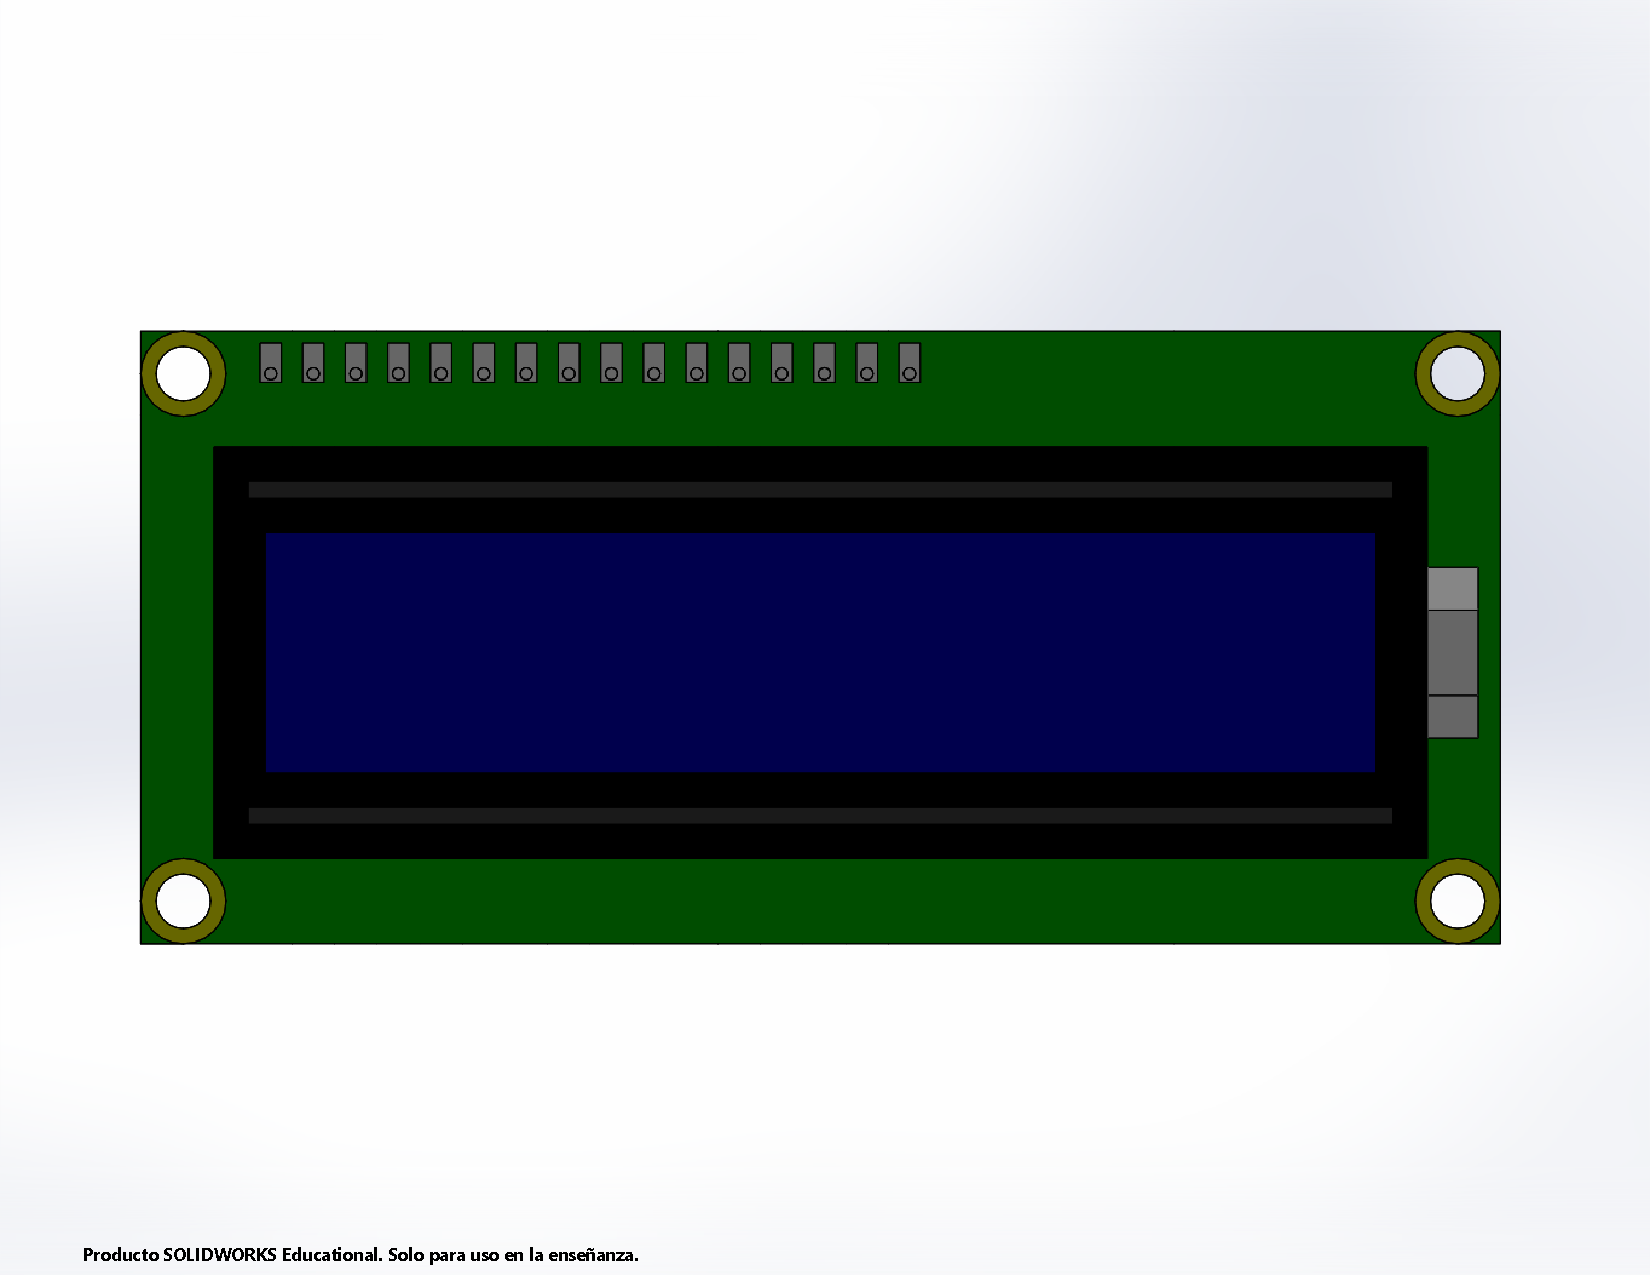
\includegraphics[trim = {1mm 20mm 1mm 20mm},clip,scale=0.2]{3/Img/lcdFigura.pdf}
        \caption{PC-04 LCD 16x2}
        \label{fig:lcdFigura}
    \end{figure}
    % 
    %
    \begin{figure}[H]
        \centering
        \includegraphics[trim = {1mm 10mm 1mm 1mm},clip,scale=0.2]{3/Img/móduloAdaptadorLcdFigura.PDF}
        \caption{PC-05 Módulo adaptador LCD 1602}
        \label{fig:móduloAdaptadorLcdFigura}
    \end{figure}
    % 
    %
    \begin{figure}[H]
        \centering
        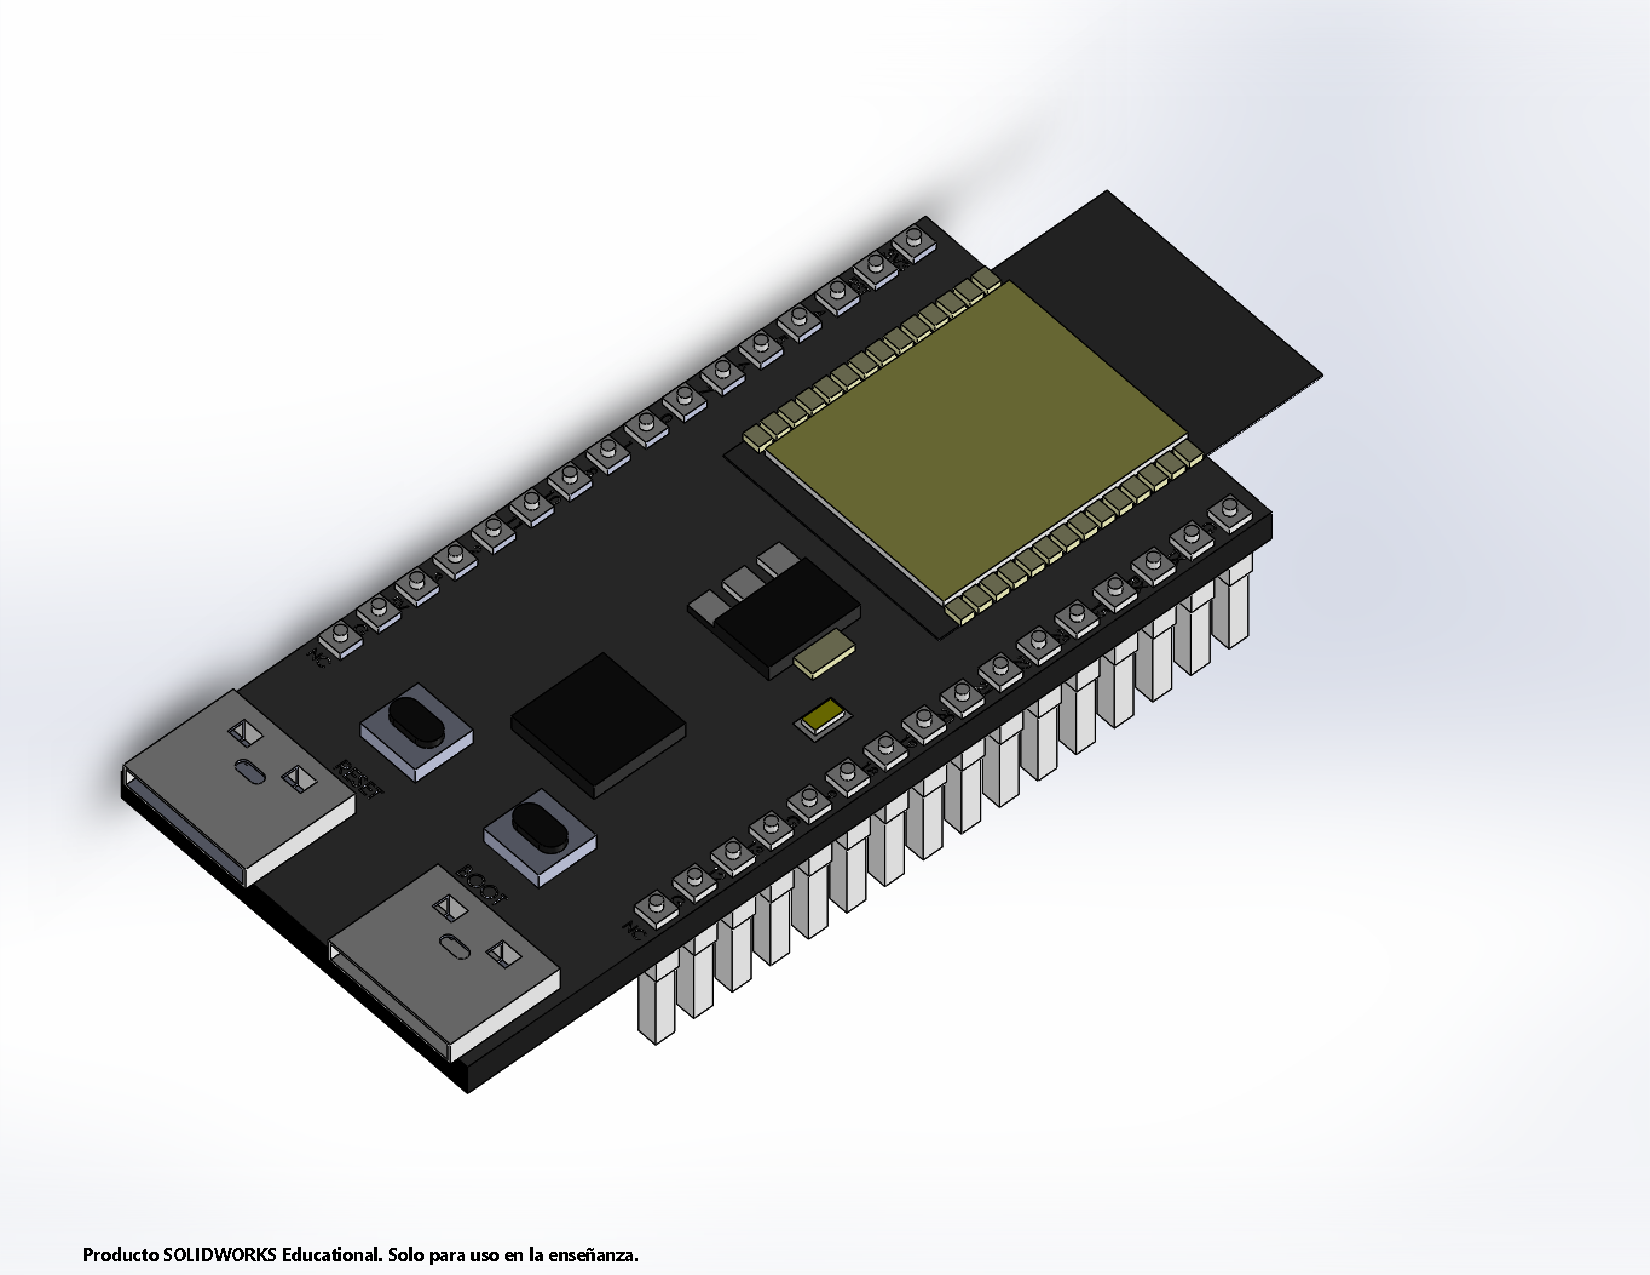
\includegraphics[trim = {1mm 10mm 20mm 1mm},clip,scale=0.2]{3/Img/esp32Figura.PDF}
        \caption{PC-06 ESP32-C6-WROOM-1}
        \label{fig:esp32Figura}
    \end{figure}
    % 
    %
    \begin{figure}[H]
        \centering
        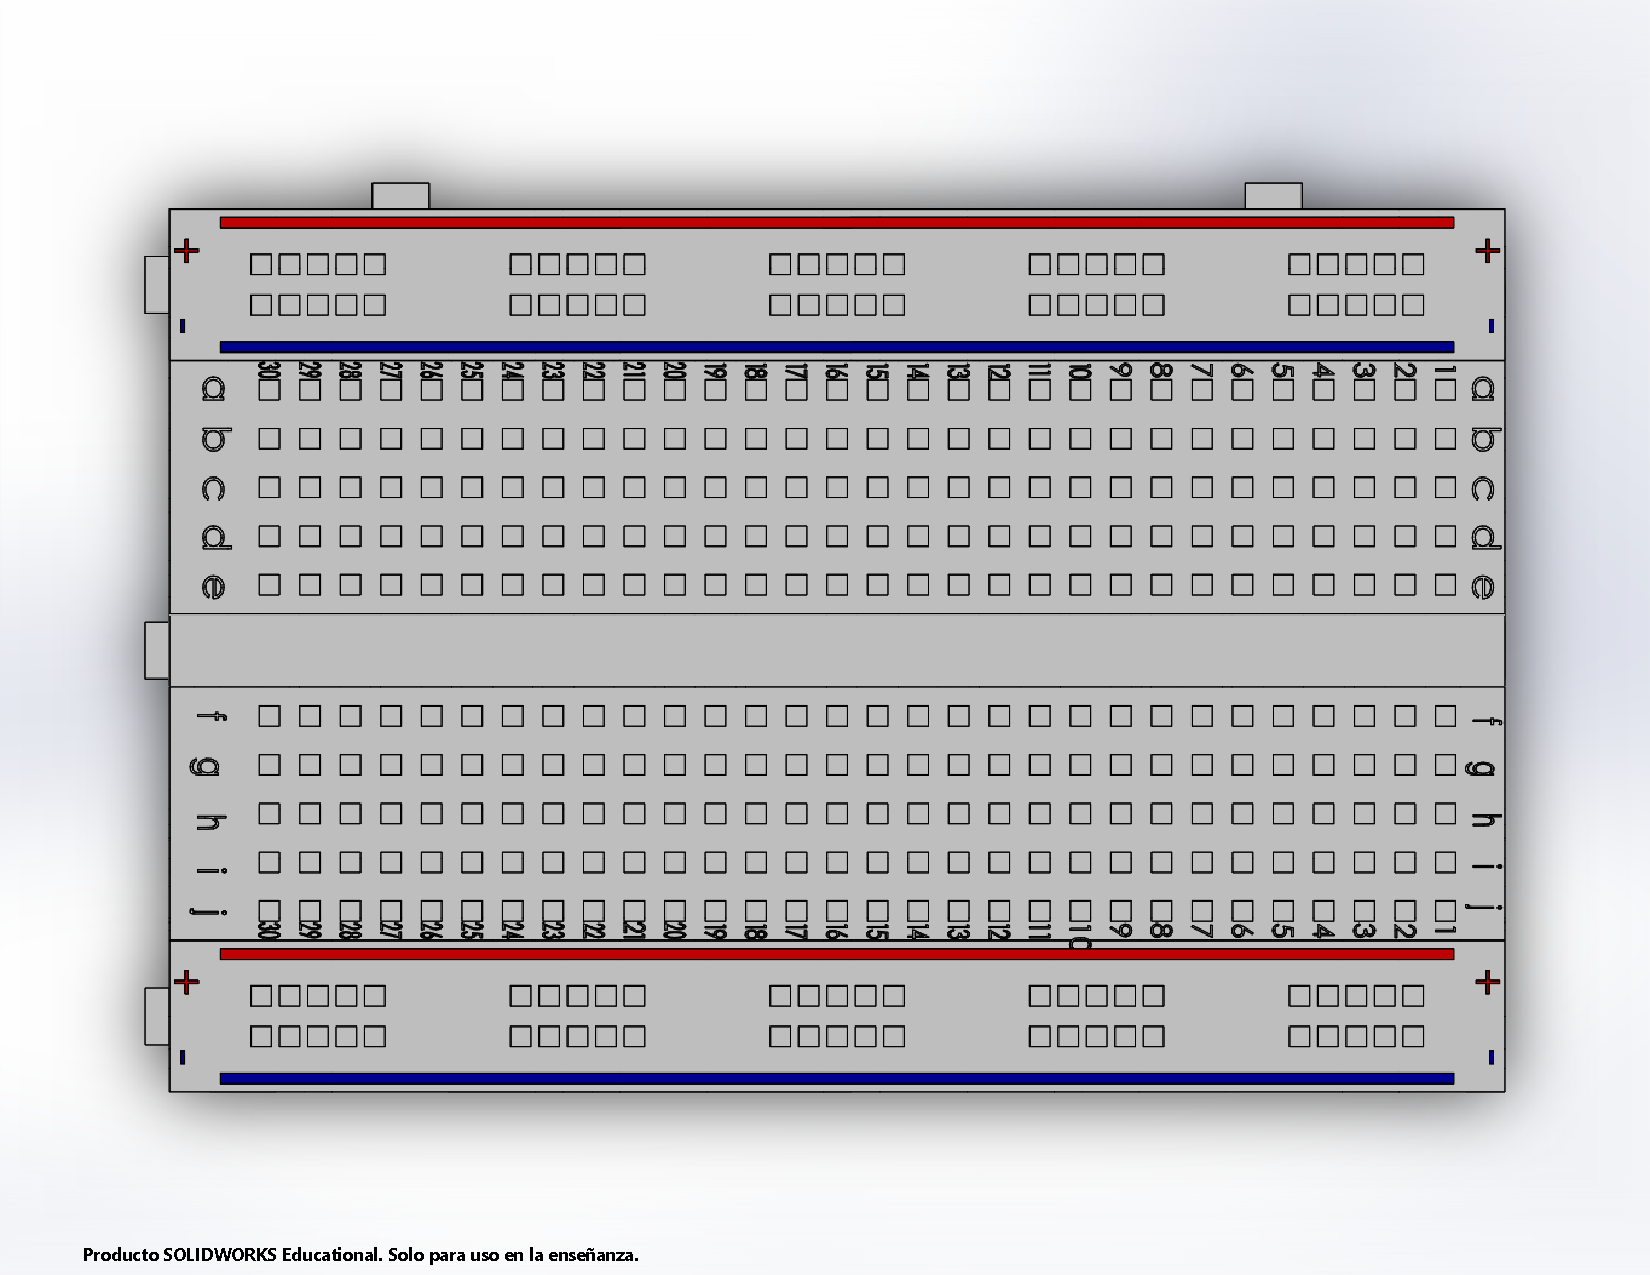
\includegraphics[trim = {1mm 10mm 1mm 1mm},clip,scale=0.2]{3/Img/protoboardFigura.PDF}
        \caption{PC-07 Protoboard}
        \label{fig:protoboardFigura}
    \end{figure}
    % 
    %
    \begin{figure}[H]
        \centering
        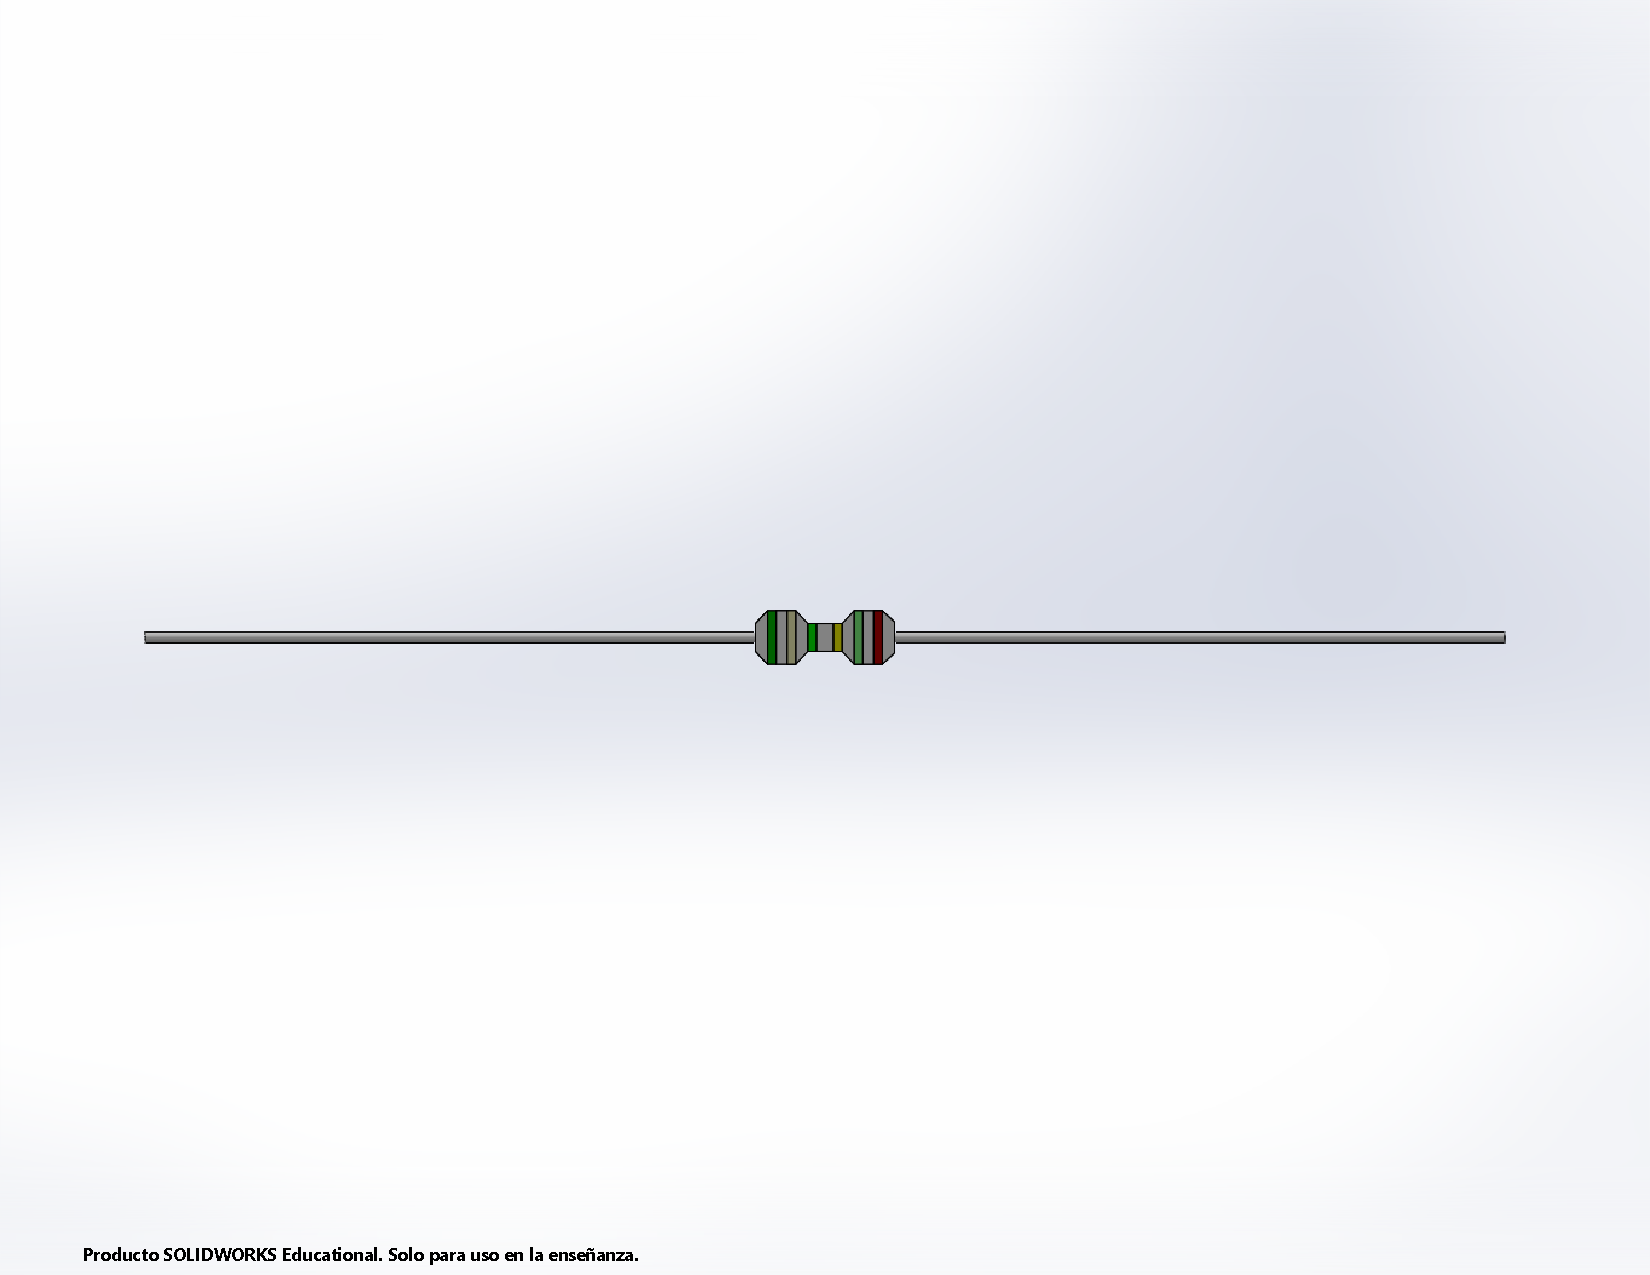
\includegraphics[trim = {1mm 50mm 1mm 50mm},clip,scale=0.2]{3/Img/resistenciaFigura.pdf}
        \caption{PC-08 Resistencia 330 1/4 W}
        \label{fig:resistenciaFigura}
    \end{figure}
    % 
    %
    \begin{figure}[H]
        \centering
        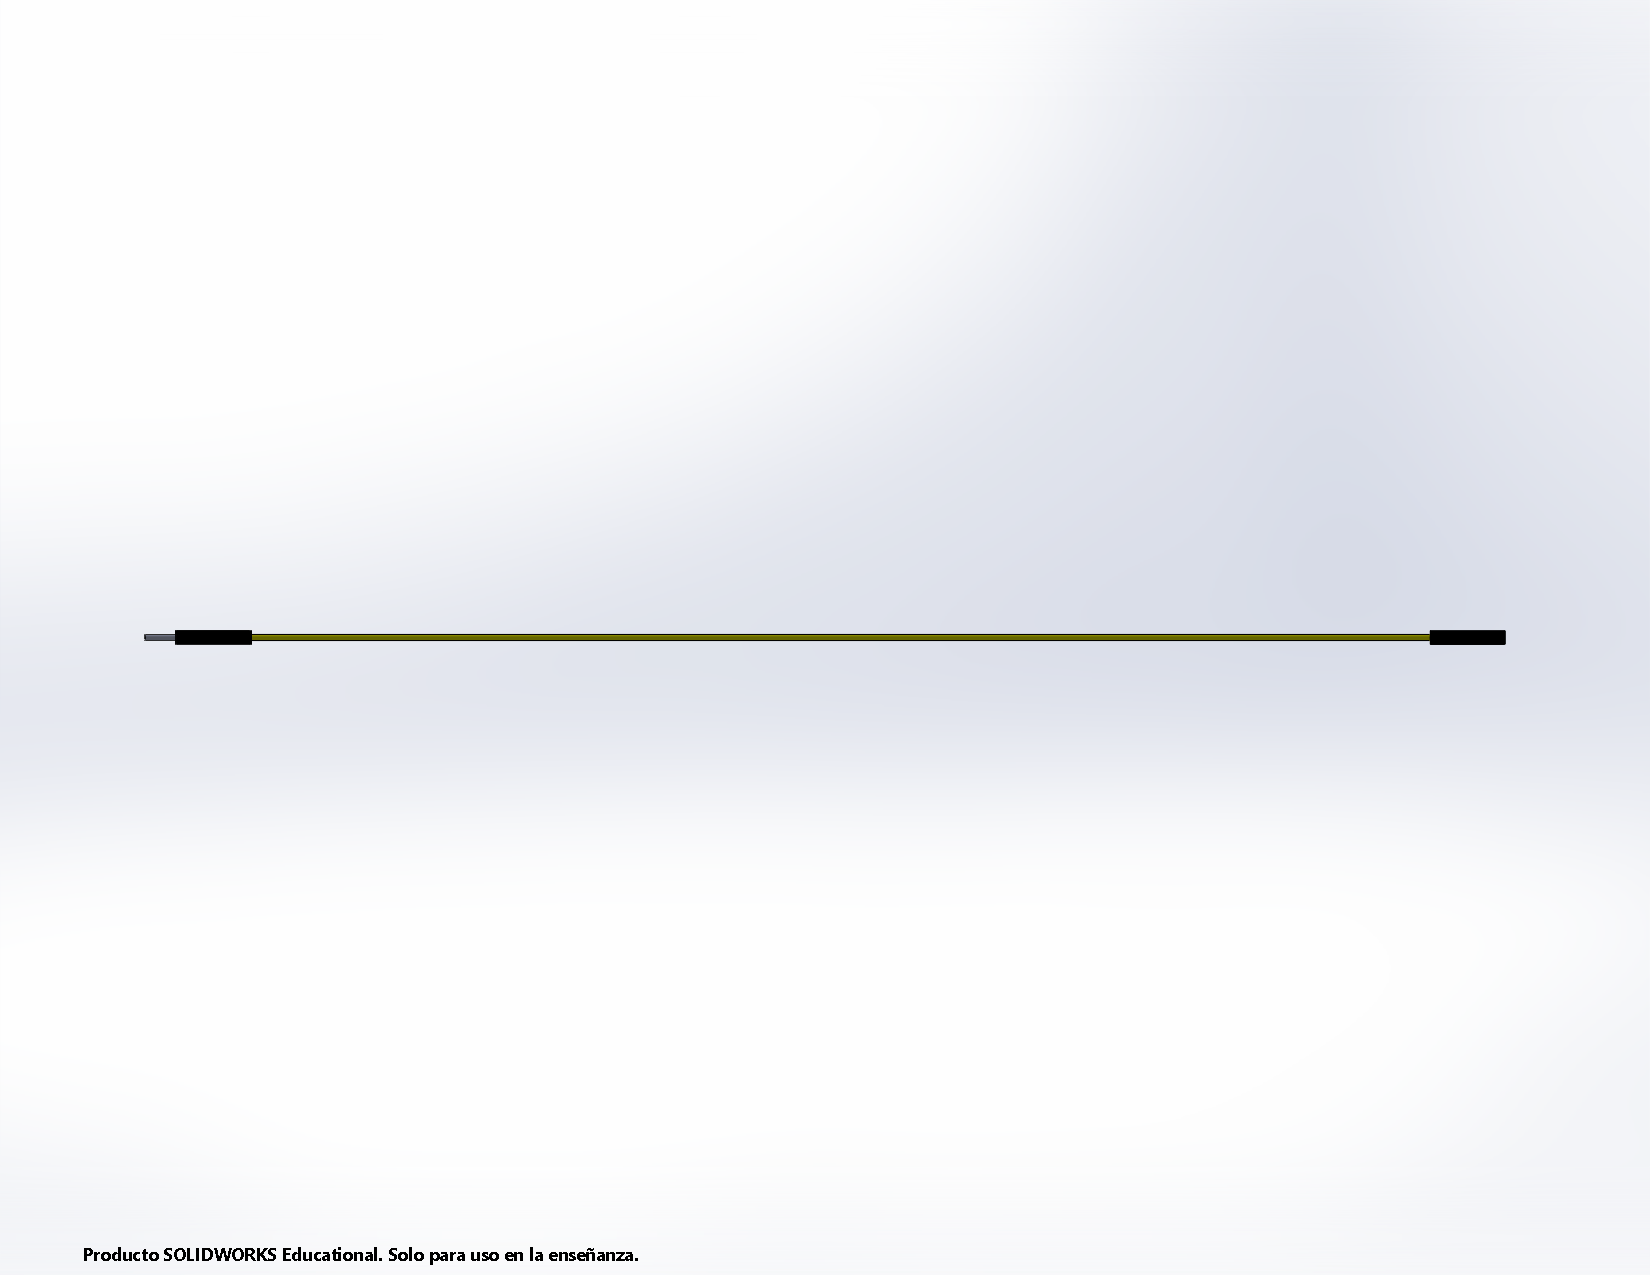
\includegraphics[trim = {1mm 50mm 1mm 50mm},clip,scale=0.2]{3/Img/cableMHFigura.pdf}
        \caption{PC-09 Cable MH 19cm}
        \label{fig:cableMHFigura}
    \end{figure}
    % 
    %
    \begin{figure}[H]
        \centering
        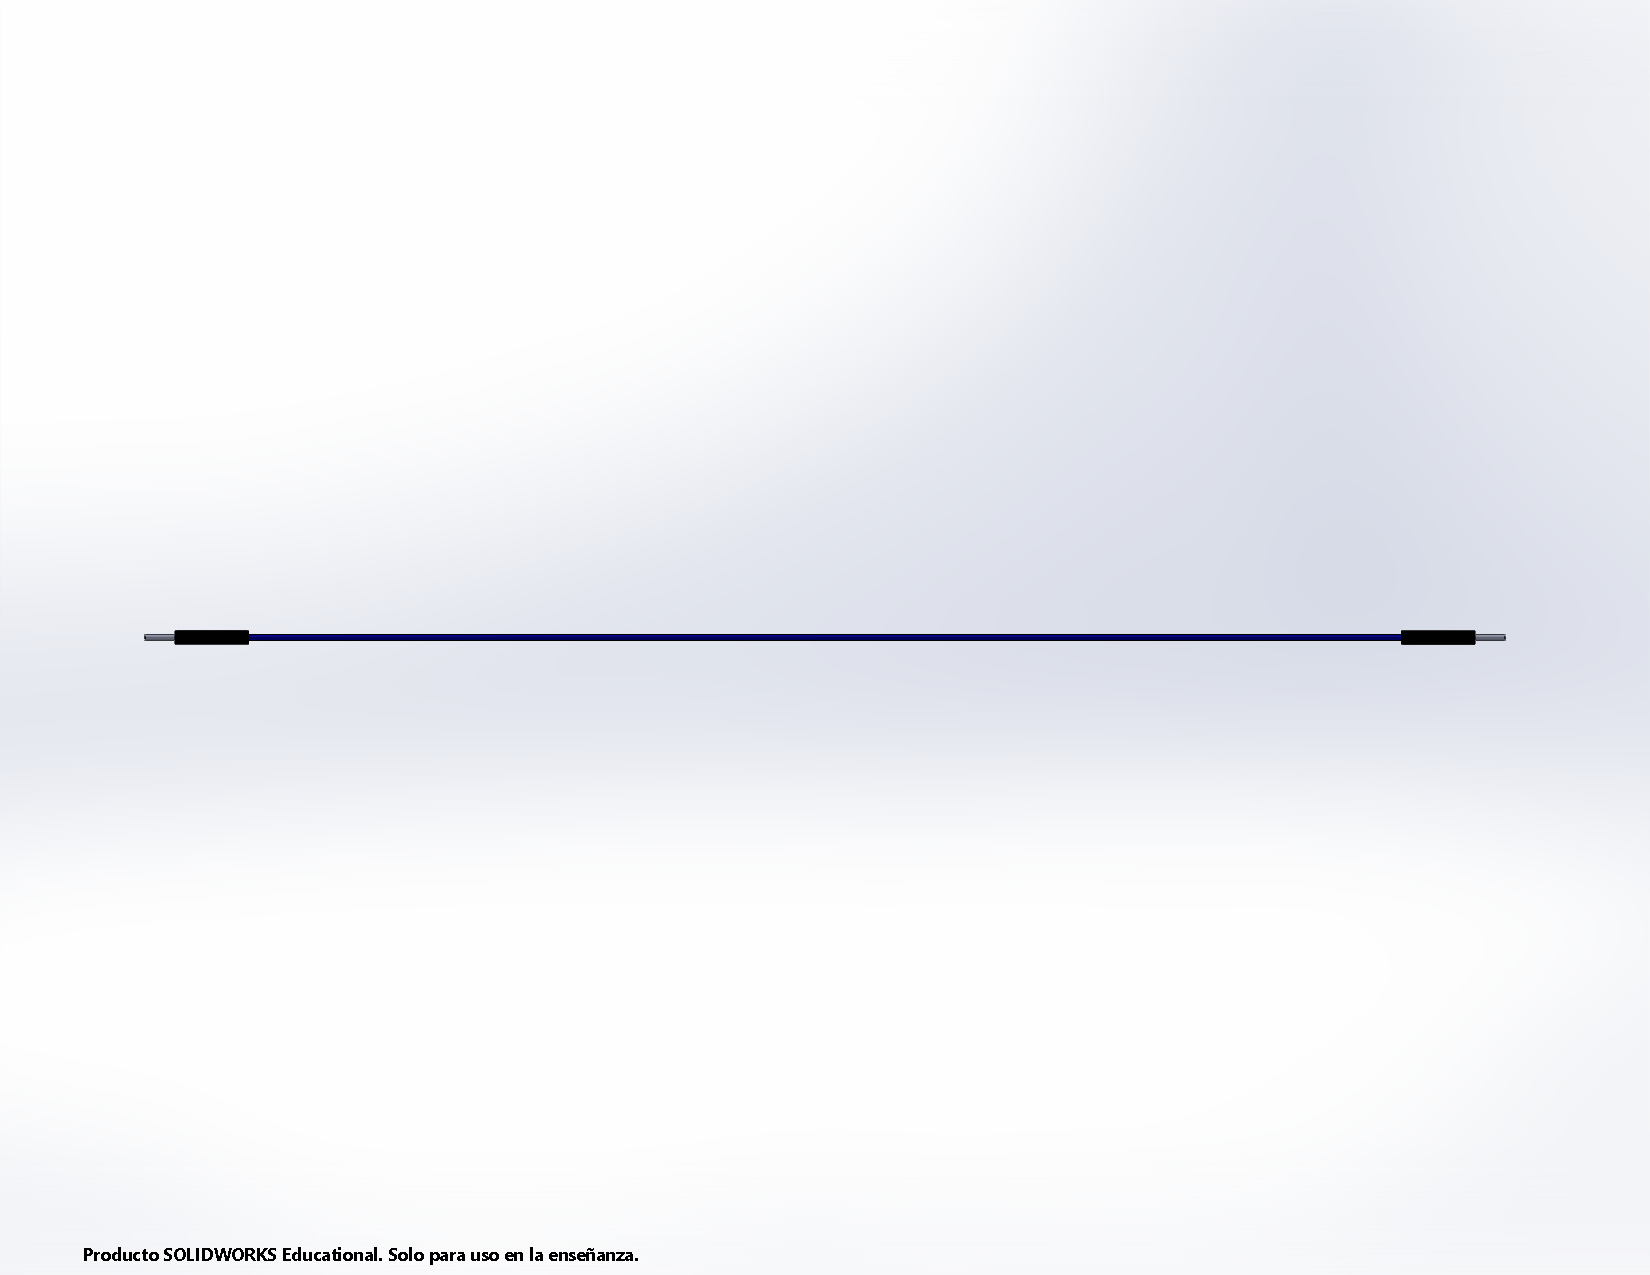
\includegraphics[trim = {1mm 50mm 1mm 50mm},clip,scale=0.2]{3/Img/cableMMFigura.pdf}
        \caption{PC-10 Cable MM 19cm}
        \label{fig:cableMMFigura}
    \end{figure}
    % 
    % 
    \begin{figure}[H]
        \centering
        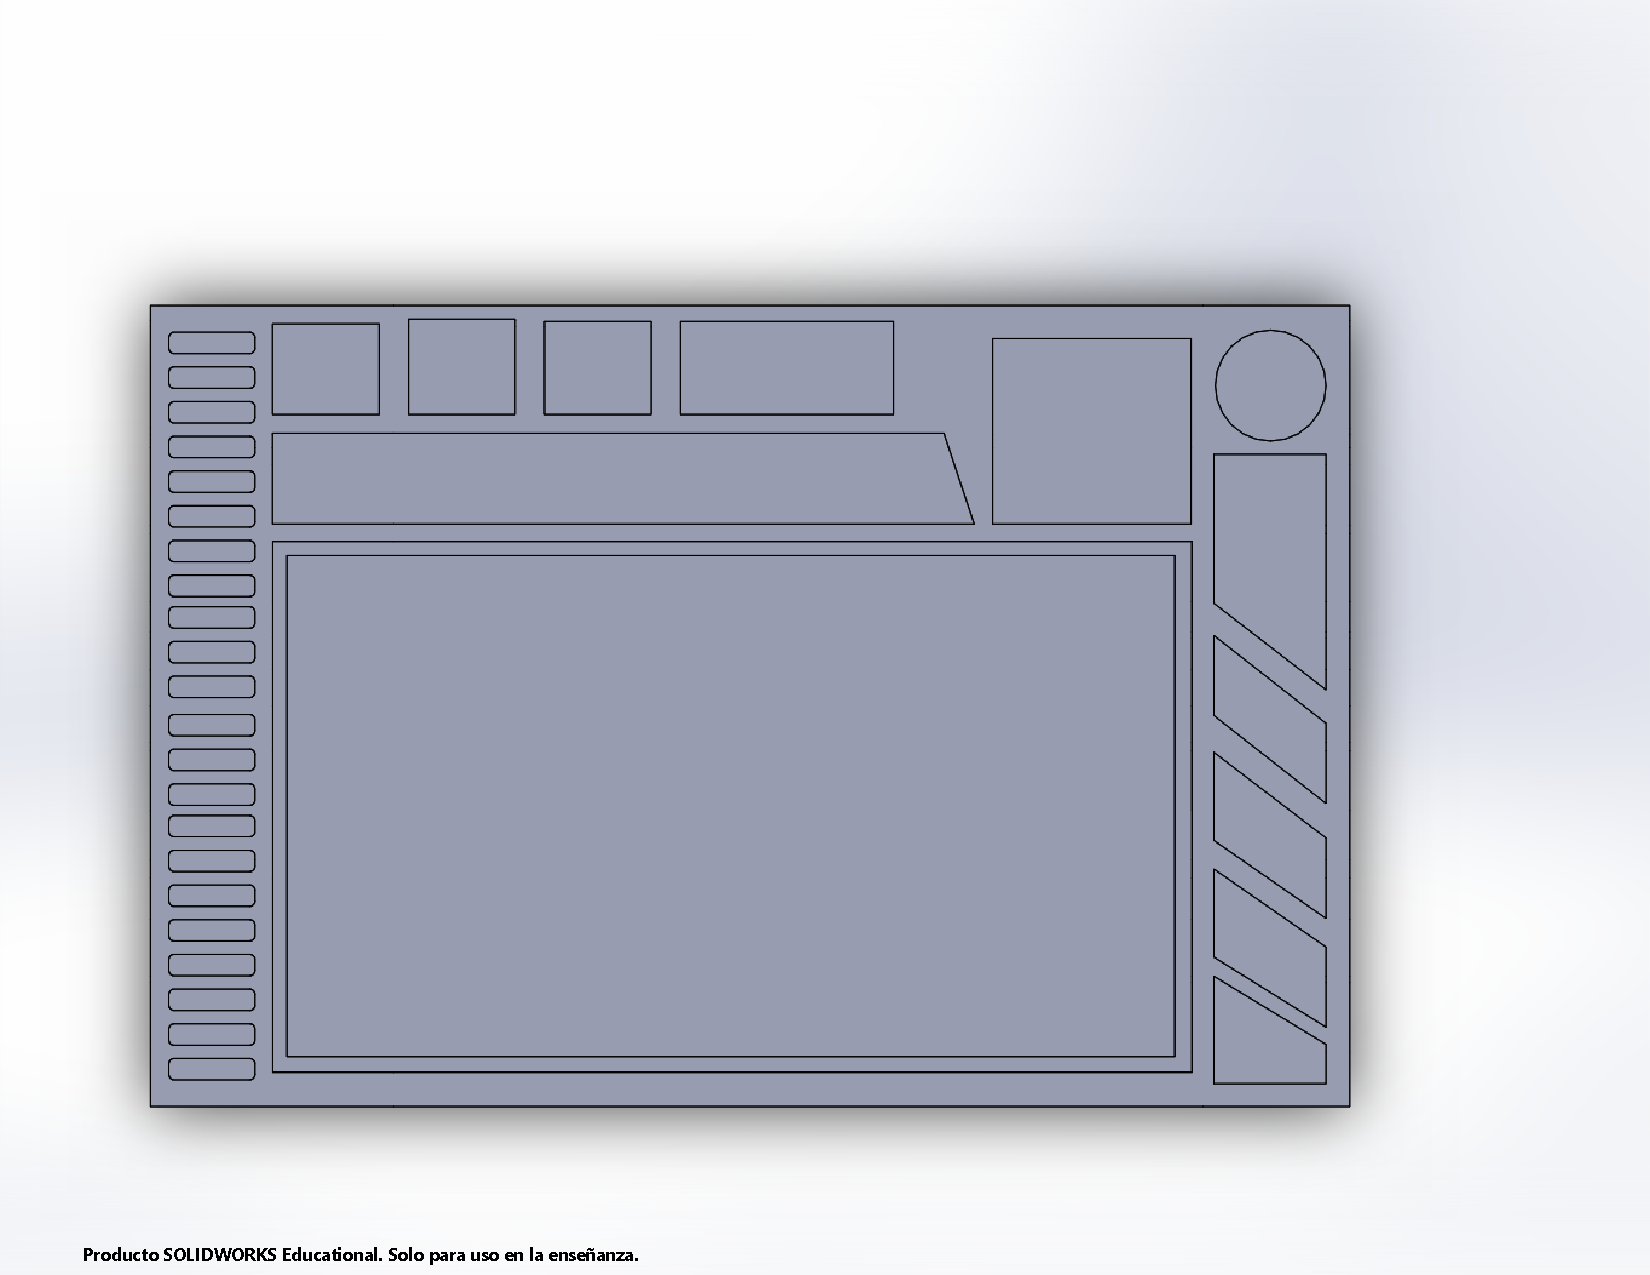
\includegraphics[trim = {1mm 10mm 30mm 30mm},clip,scale=0.2]{3/Img/tapeteProfesionalOrganizadorDeTrabajoFigura.pdf}
        \caption{PC-11 Tapete profesional organizador de trabajo}
        \label{fig:tapeteProfesionalOrganizadorDeTrabajoFigura}
    \end{figure}
    % 
    % 
    \subsection{Prepara tu documento}
    
    Antes de que comiences a utilizar esta plantilla, es recomendable que prepare la información que contendrá en un archivo aparte. 
    Ten preparadas tus gráficas, así como también las tablas aparte, para que sea más fácil integrarlo. 
    Se recomienda fuertemente el uso de \textbf{formato Enhanced Metafile (.emf) para imágenes y gráficas} de resolución óptima. 
    Finalmente, completa y organiza el contenido antes de darle el formato de esta plantilla. 
    
    \subsection{Acrónimos y Abreviaciones}
    
    Los acrónimos y abreviaciones deberán ser definidos únicamente la primera vez que aparecen en el texto, esto para que el lector entienda lo que significan.
    
    \subsection{Ecuaciones}
    
    Las ecuaciones son una excepción a las especificaciones prescritas de esta plantilla. 
    Deberá determinar si su ecuación debe escribirse o no utilizando la fuente Adobe Devangari. 
    Para crear ecuaciones multinivel, puede ser necesario tratar la ecuación como un gráfico e insertarla en el texto después de aplicar el estilo de la platilla.
    Las ecuaciones serán enumeradas de manera consecutiva, y el número de ecuación, entre paréntesis, se colocan al ras de la derecha, utilizando una tabulación derecha. 
    
    \begin{equation}
        \label{eq1}
        x + y = z 
    \end{equation}
    
    Es importante asegurarse de que los símbolos de la ecuación sean definidos antes o inmediatamente después de la ecuación. Utilice “(1)”, en vez de “Eq. 1” al enumerar las ecuaciones, excepto al principio de una oración: “La ecuación (\ref{eq1}) es…”
    
    \section{Resultados y discusión}
    
    Antes de comenzar a preparar tu artículo, es importante que lea primero la guía del autor, la cual incluye los temas o apartados que son necesarios para tener tu trabajo completo.
    Una vez completada la edición del texto, el documento está listo para el uso de esta plantilla. En este archivo recién creado, resalte todo el contenido e importe el archivo de texto preparado. Ahora esta listo para estilizar su documento.
    En esta sección se deben presentar todo lo obtenido de la sección 2, incluidas deducciones o efectos del desarrollo. También se podrán incluir subsecciones numeradas de la siguiente forma:
    
    \subsection{Autores y Afiliaciones}
    
    Para distinguir las afiliaciones de los autores, utilice superíndices iniciando con el número 1, 2, etc., sucesivamente, esto dependerá de la cantidad de los departamentos a los que estén afiliados los autores. En caso de que todos los autores pertenezcan a una mismo departamento e institución, utilizar sólo el superíndice 1. 
    
    \subsection{Identificar los encabezados}
    
    Se les recuerda a los autores que los encabezados deben de estar conforme los solicita la guía del autor. De ahí se puede adaptar el trabajo para que sea más fácil de entender para el lector.
    Los encabezados organizan los temas sobre una base relacional y jerárquica. Por ejemplo, el título del documento es encabezado del texto principal porque todo el material posterior se relaciona y elabora sobre este tema. 
    
    \subsection{Tablas y Figuras}
    
    \begin{enumerate}
        \item Posición de las tablas y figuras: Coloque las figuras y las tablas en la parte superior e inferior de las columnas. Evite colocarlos en medio. Las figuras y las tablas grandes pueden abarcar ambas columnas. Los títulos de las figuras deben de estar debajo de las mismas; los títulos de las tablas deben aparecer encima de ellas. Insértese las figuras y los cuadros después de citarse en el texto. Utilice la abreviatura “Fig. 1”, incluso al principio de una oración. 
    \end{enumerate}
    
    \section{Conclusiones}
    
    Se describe aquí el alcance del trabajo, logros obtenidos y perspectivas para el futuro de este. Se sugiere colocar información cuantitativa obtenida.
    
    \section{Agradecimientos}
    
    Es importante darles su debido reconocimiento a los laboratorios, instituciones, organizaciones, entre otros que han sido participes para la culminación de este trabajo. También es importante mencionar, fondos, proyectos, becas, entre otros que se le han otorgado al o los autores para realizar el trabajo de investigación. Ejemplo: “Los autores agradecen al Concejo Nacional de Ciencia y Tecnología por los recursos otorgados…”
    
    \section*{Referencias}
    
    % Para esta platilla, se solicita al autor enumerar las citas de manera consecutiva entre corchetes \cite{YLi2013}. 
    % La puntuación de la oración que sigues sería \cite{Mesaelides2011}. 
    % Refiérase simplemente al número de referencia, como en \cite{Morales2012}, no utilice “Ref. [3]” o “referencia [3]” excepto al principio de una oración: “La referencia [3] fue la primera…”
    Enumere las notas al pie por separado en superíndices. Coloque la nota de pie de en la parte inferior de la columna en la que se citó. No coloque notas al pie en la lista de referencias. Utilice letras para las notas al pie de la tabla.
    A menos de que haya tres autores o más; no utilice “et al.”. Los trabajos que no hayan sido publicados, incluso si han sido presentados para su publicación, deben ser citados como “inéditos”. Los trabajos que han sido aceptados para su publicación deben de citarse como “en prensa”. Poner en mayúscula sólo la primera palabra de un título, excepto los nombres propios y los símbolos de elemento. 
    % Otros ejemplos \cite{LAAngeles2021}, \cite{LAAngelesConni}. 
    % Véase el archivo adjunto \ref{anexo:pines}.
    
    % Ejemplo
    %  @Article{article,
    % 	author = "Author1 LastName1 and Author2 LastName2 and Author3 LastName3",
    % 	title = "Article Title",
    % 	volume = "30",
    % 	number = "30",
    % 	pages = "10127-10134",
    % 	year = "2013",
    % 	doi = "10.3389/fnins.2013.12345",
    % 	URL = "http://www.frontiersin.org/Journal/10.3389/fnins.2013.12345/abstract",
    % 	journal = "Frontiers in Neuroscience"
    % }
    
    % @book{book,
    %   author    = {Author Name}, 
    %   title     = {The title of the work},
    %   publisher = {The name of the publisher},
    %   address   = {The city},
    %   year      = 1993,
    % }
    
    % @incollection{chapter,
    %   author       = {Bauthor Surname}, 
    %   title        = {The title of the work},
    %   editor       = {Editor Name},
    %   booktitle    = {The title of the book},
    %   publisher    = {The name of the publisher},
    %   address      = {The city},
    %   year         = 2002,
    %   pages        = {201-213},
    % }
    
    % @InProceedings{conference,
    %   author = {Cauthor Name and Dauthor Surname and Fauthor LastName},
    %   title = {The title of the work},
    %   booktitle = {The title of the conference proceedings},
    %   year = 1996,
    %   publisher = {The name of the publisher},
    %   editor = {Editor Name1 and Editor Name2},
    %   pages = {41-50},
    % }
    
    % @book{cho,
    %   author       = {Gauthor Name1}, 
    %   title        = {The title of the work},
    %   publisher = {Country code and patent number},
    %   address      = {Patent Country},
    %   year = 2013
    % }
    
    % @book{patent,
    %   author    = {Hauthor Surname1}, 
    %   title     = {The title of the work},
    %   publisher = {Patent number},
    %   address   = {Patent country},
    %   year      = 2010,
    % }
    
    % % please use misc for datasets
    % @misc{dataset, 
    % 	author = "Author1 LastName1 and Author2 LastName2 and Author3 LastName3",
    % 	title = "Data Title",
    % 	year = "2011",
    % 	doi = "10.000/55555",
    % 	URL = "http://www.frontiersin.org/",
    % }
    % 
    % 
    \bibliographystyle{ieeetr}
    \bibliography{3/referencias}
    %
    %
    %%%%%%%%%%%%%%%%%%%%%%%%%%%%%%%%%%
    \appendix
    %%%%%%%%%%%%%%%%%%%%%%%%%%%%%%%%%%
    % 
    % 
    \centering{\section[\appendixautorefname{}]{HOJA DE REGISTRO}}\label{anexo:hojaDeRegistro }
    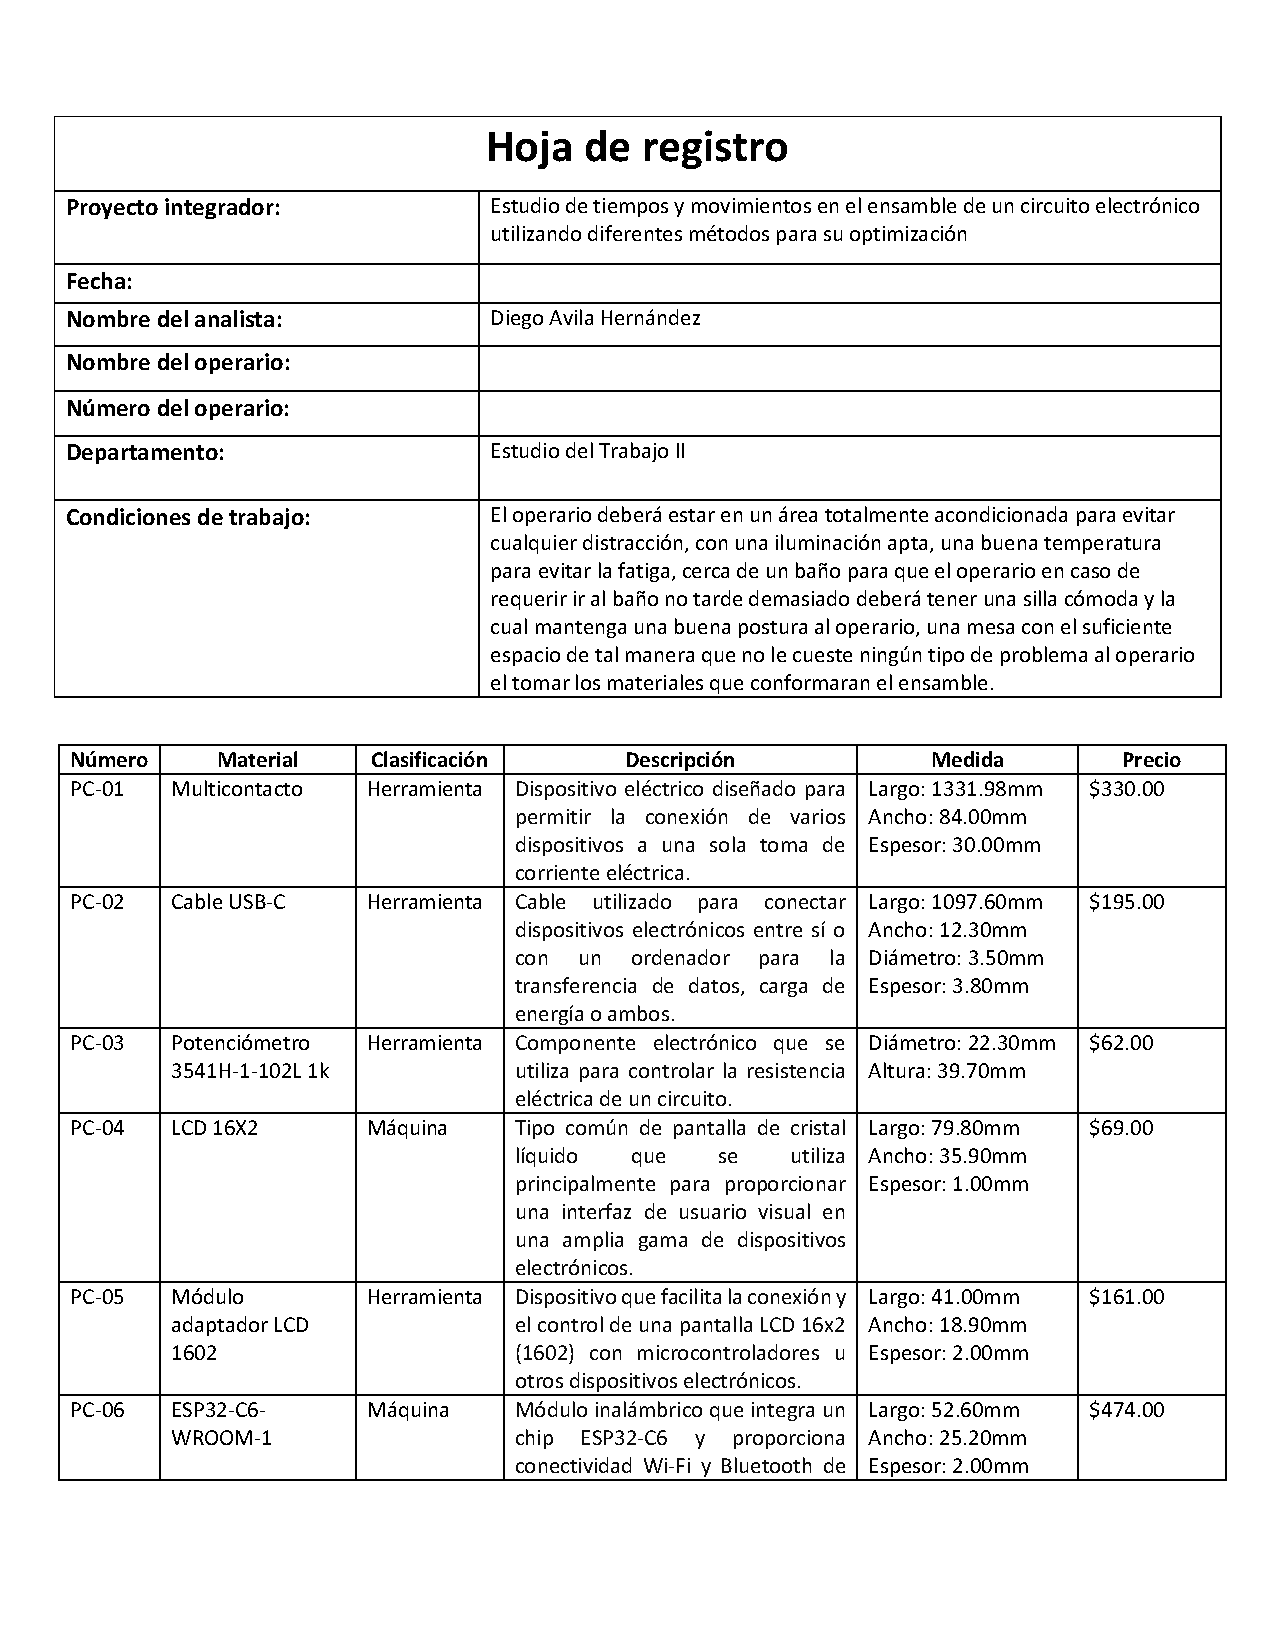
\includepdf[pages=-]{3/Img/hojaDeRegistro .pdf}
    %%%%%%%%%%%%%%%%%%%%%%%%%%%%%%%%%%%%%%%%
    % 
    % 
    %%%%%%%%%%%%%%%%%%%%%%%%%%%%%%%%%%
    \appendix
    %%%%%%%%%%%%%%%%%%%%%%%%%%%%%%%%%%
    % 
    % 
    \centering{\section[\appendixautorefname{}]{}}\label{anexo:ensambleDeCircuitoElectrónico}
    \includepdf[pages=-]{3/Img/ensambleDeCircuitoElectrónico.pdf}
    %%%%%%%%%%%%%%%%%%%%%%%%%%%%%%%%%%%%%%%%